% Created 2017-09-19 Tue 15:40
% Intended LaTeX compiler: pdflatex
\documentclass[11pt]{article}
\usepackage[utf8]{inputenc}
\usepackage[T1]{fontenc}
\usepackage{graphicx}
\usepackage{grffile}
\usepackage{longtable}
\usepackage{wrapfig}
\usepackage{rotating}
\usepackage[normalem]{ulem}
\usepackage{amsmath}
\usepackage{textcomp}
\usepackage{amssymb}
\usepackage{capt-of}
\usepackage{hyperref}
\author{Francesco Ferraro, Diego Batista, Leonardo Martins}
\date{\today}
\title{T1 Autômatos}
\hypersetup{
 pdfauthor={Francesco Ferraro, Diego Batista, Leonardo Martins},
 pdftitle={T1 Autômatos},
 pdfkeywords={},
 pdfsubject={},
 pdfcreator={Emacs 25.1.2 (Org mode 9.0.10)}, 
 pdflang={English}}
\begin{document}

\maketitle
\begin{abstract}
Entrega formal do primeiro trabalho da disciplina de automatos na PUCRS.
\end{abstract}

\section{Questão 1}
\label{sec:org8beb6a2}

\subsection{Cadeias que terminam por bcb}
\label{sec:org1c37157}
\begin{figure}[htbp]
\centering
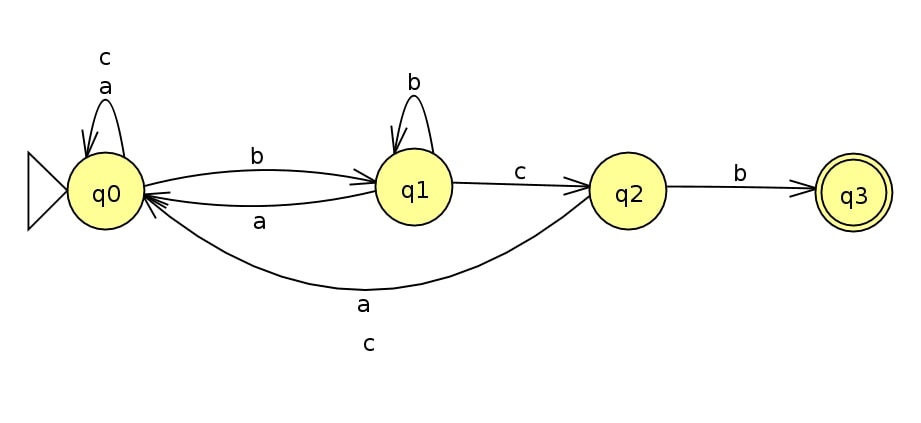
\includegraphics[width=.9\linewidth]{./q1/a/q1a.jpg}
\caption{\label{fig:orgb1c2188}
Esse é um autômato determinístico}
\end{figure}

\begin{center}
\begin{tabular}{ll}
Input & Result\\
\hline
abcb & Accept\\
bcbb & Reject\\
cbcb & Accept\\
bcbaaa & Reject\\
aaaaa & Reject\\
\end{tabular}
\end{center}

\subsection{Cadeias que terminam por no máximo dois b´s}
\label{sec:org22d783e}
\begin{figure}[htbp]
\centering
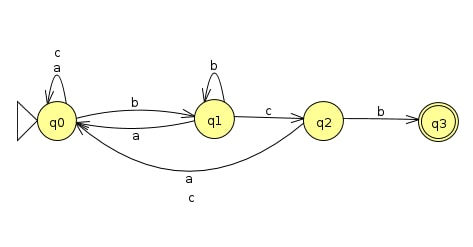
\includegraphics[width=.9\linewidth]{./q1/b/q1b.jpg}
\caption{\label{fig:org8c4e505}
Esse é um autômato determinístico}
\end{figure}

\begin{center}
\begin{tabular}{ll}
Input & Result\\
\hline
b & Reject\\
a & Reject\\
c & Reject\\
bb & Reject\\
aba & Reject\\
ac & Reject\\
ab & Reject\\
bc & Reject\\
ba & Reject\\
\end{tabular}
\end{center}
\subsection{Cadeias que não terminam por dois bs consecutivos}
\label{sec:orge5009bf}
\begin{figure}[htbp]
\centering
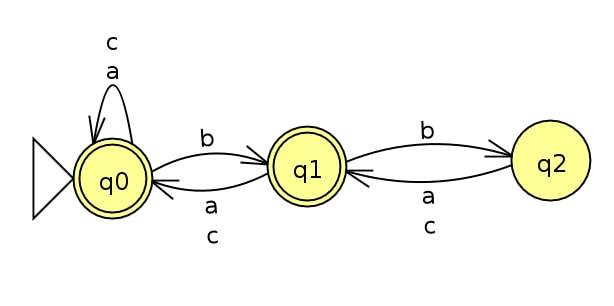
\includegraphics[width=.9\linewidth]{./q1/c/q1c.jpg}
\caption{\label{fig:org83f78cf}
Esse é um autômato determinístico}
\end{figure}

\begin{center}
\begin{tabular}{ll}
Input & Result\\
\hline
aa & Accept\\
bb & Reject\\
cc & Accept\\
c & Accept\\
a & Accept\\
b & Accept\\
aacbac & Accept\\
abcabc & Reject\\
\end{tabular}
\end{center}
\subsection{Cadeias que iniciam por a e terminam com c}
\label{sec:org71ce23b}
\begin{figure}[htbp]
\centering
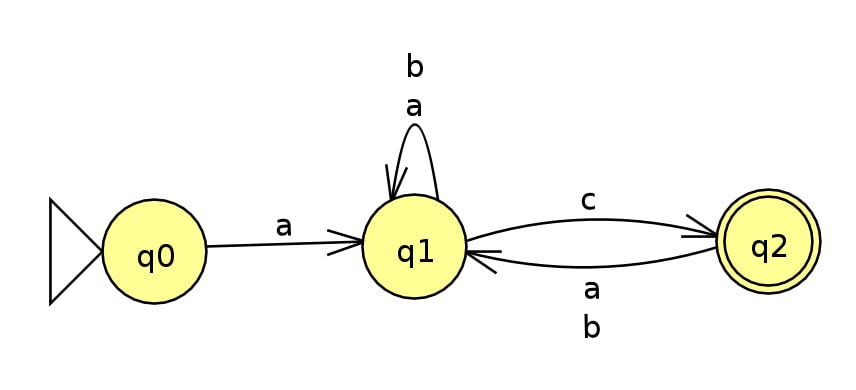
\includegraphics[width=.9\linewidth]{./q1/d/q1d.jpg}
\caption{\label{fig:orgc663817}
Esse é um autômato determinístico}
\end{figure}

\begin{center}
\begin{tabular}{ll}
Input & Result\\
\hline
a & Reject\\
b & Reject\\
c & Reject\\
ac & Accept\\
abcbc & Accept\\
acac & Accept\\
abcbb & Reject\\
\end{tabular}
\end{center}
\subsection{Cadeias que iniciam e terminam pelo mesmo símbolo}
\label{sec:org08d886f}
\begin{figure}[htbp]
\centering
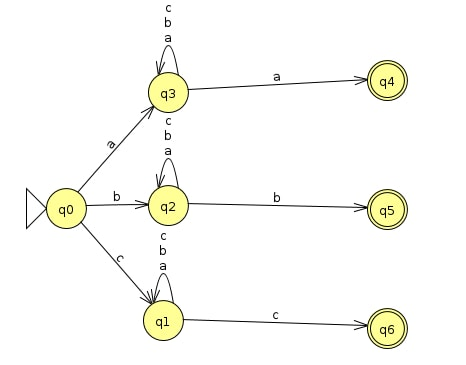
\includegraphics[width=.9\linewidth]{./q1/e/q1e.jpg}
\caption{\label{fig:org0b80950}
Esse é um autômato determinístico}
\end{figure}

\begin{center}
\begin{tabular}{ll}
Input & Result\\
\hline
aa & Accept\\
bb & Accept\\
cc & Accept\\
ac & Reject\\
ab & Reject\\
bbaa & Reject\\
bba & Reject\\
\end{tabular}
\end{center}
\subsection{Cadeias que iniciam e terminam por símbolos diferentes}
\label{sec:org5c8329a}

\begin{figure}[htbp]
\centering
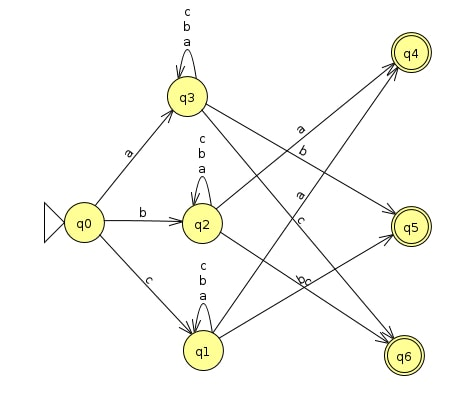
\includegraphics[width=.9\linewidth]{./q1/f/q1f.jpg}
\caption{\label{fig:org9a5945c}
Esse é um autômato determinístico}
\end{figure}

\begin{center}
\begin{tabular}{ll}
Input & Result\\
\hline
aa & Reject\\
bb & Reject\\
cc & Reject\\
ac & Accept\\
ab & Accept\\
bbaa & Accept\\
bba & Accept\\
abcbcba & Reject\\
\end{tabular}
\end{center}

\subsection{Cadeias que tenham um número ímpar de b’s}
\label{sec:orgbe6e89a}
\begin{figure}[htbp]
\centering
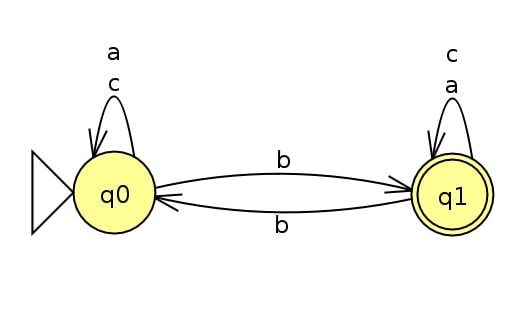
\includegraphics[width=.9\linewidth]{./q1/g/q1g.jpg}
\caption{\label{fig:orgd79cf0a}
Esse é um autômato determinístico}
\end{figure}

\begin{center}
\begin{tabular}{ll}
Input & Result\\
\hline
aa & Reject\\
bb & Reject\\
cb & Accept\\
ac & Reject\\
ab & Accept\\
bbaa & Reject\\
bba & Reject\\
abcbcba & Accept\\
b & Accept\\
\end{tabular}
\end{center}

\section{Questão 2}
\label{sec:org4f35ea8}
\section{Questão 3}
\label{sec:org253fa08}
\subsection{Automato}
\label{sec:org88a6f76}
A figura \ref{fig:org97f3017} reponde essa questão. 

\begin{figure}[htbp]
\centering
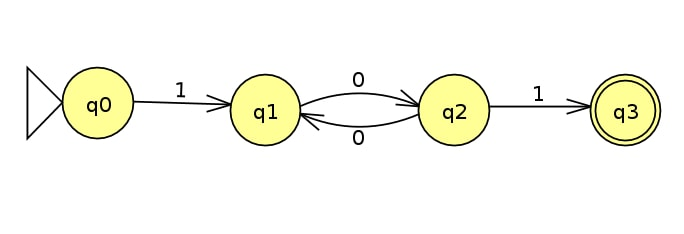
\includegraphics[width=.9\linewidth]{./q3/q3.jpg}
\caption{\label{fig:org97f3017}
Esse é um autômato determinístico}
\end{figure}

A tabela abaixo confirma o automato na figura \ref{fig:org97f3017}. 

\begin{center}
\begin{tabular}{rl}
Input & Result\\
\hline
0 & Reject\\
01 & Reject\\
1 & Reject\\
101 & Accept\\
1001 & Reject\\
10001 & Accept\\
100001 & Reject\\
1000001 & Accept\\
10000001 & Reject\\
\end{tabular}
\end{center}
\subsection{Expressão regular}
\label{sec:org0f57cbb}

\textbf{10+(00)*+1} 
\section{Questão 4}
\label{sec:orgbfafa96}
\begin{figure}[htbp]
\centering
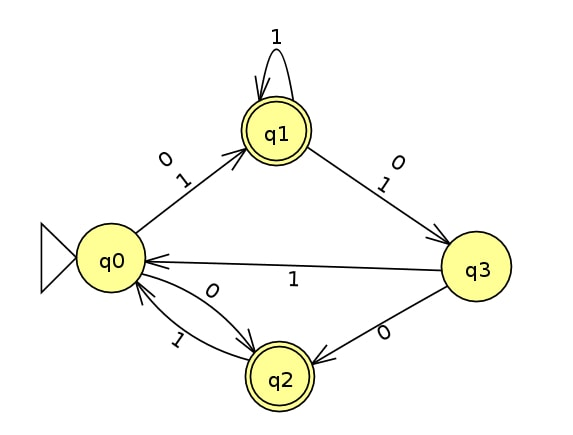
\includegraphics[width=.9\linewidth]{./q4/q4.jpg}
\caption{\label{fig:orgf34a0a2}
Esse é um autômato determinístico}
\end{figure}
\section{Questão 5}
\label{sec:org66fad5b}
\section{Questão 6}
\label{sec:orgd9d624a}
\subsection{Estacionamento}
\label{sec:org89b4549}
Resposta é a figura \ref{fig:org48f1e65}.
\begin{figure}[htbp]
\centering
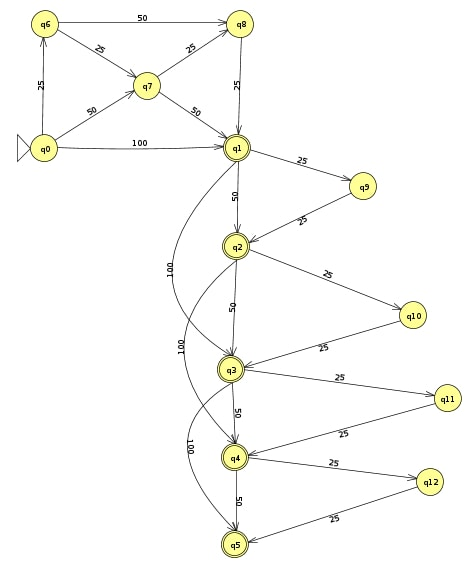
\includegraphics[width=.9\linewidth]{./q6/estacionamento.jpg}
\caption{\label{fig:org48f1e65}
Autômato de uma parquímetro}
\end{figure}
\section{Questão 7}
\label{sec:orgf65ba71}
\end{document}
